%--------------------------------------------------------------------------
%	PACKAGES AND OTHER DOCUMENT CONFIGURATIONS
%--------------------------------------------------------------------------
\documentclass[11pt,a4paper]{article}
\usepackage[utf8]{inputenc}
\usepackage[english]{babel}
\usepackage[T1]{fontenc}
\usepackage{amsmath}
\usepackage{mathtools}
\usepackage{amsfonts}
\usepackage{amssymb}
\usepackage{pifont}% http://ctan.org/pkg/pifont
\usepackage{graphicx}
\usepackage{epstopdf}
\usepackage{lmodern}
\usepackage[left=3cm,right=3cm,top=2.5cm,bottom=2.5cm]{geometry}

\usepackage{fancyhdr} % Required for custom headers
\usepackage{lastpage} % Required to determine the last page for the footer
\usepackage{extramarks} % Required for headers and footers
%\usepackage[usenames,dvipsnames]{color} % Required for custom colors
\usepackage[usenames,dvipsnames]{xcolor}
\usepackage{graphicx} % Required to insert images
\usepackage{caption}
\usepackage{subcaption}
\usepackage{listings} % Required for insertion of code
%\usepackage{courier} % Required for the courier font
\usepackage{verbatim}
\usepackage{multirow}
\usepackage{eurosym}
\usepackage{url}
\usepackage{hyperref}
\usepackage[outline]{contour}
 \contourlength{.5pt}
\usepackage[noadjust]{cite}
\usepackage{tabularx}

\usepackage{enumerate}
\usepackage{enumitem}
\setlist[itemize]{noitemsep, topsep=0pt, label={---}}
\usepackage{todonotes}
%\usepackage{relsize}

\usepackage{tikz}
\usetikzlibrary{matrix}

\setlength\parindent{0pt} % Removes all indentation from paragraphs
\setlength{\parskip}{10pt plus 1pt minus 1pt}

%\definecolor{bleu}{HTML}{0000FF}
%\definecolor{jaune}{HTML}{EDB601}
%\definecolor{vert}{HTML}{008E45}
%\definecolor{rouge}{HTML}{FF0000}

%\renewcommand\thesection{\Roman{section}}

\begin{document}
	
%--------------------------------------------------------------------------
%	TITLE PAGE
%--------------------------------------------------------------------------
\begin{center}
{\bfseries
Linköping University\\
TDDD17 Information Security, Second Course\\

Lab 1: Authentication with OpenID\\
Lab assistant: Ulf Kargén\\[10pt]}

Guillaume Lambert (guila302) and Lena Peschke (lenpe782)\\
version 1, 15-01-27
\end{center}

\hrulefill

%--------------------------------------------------------------------------
%	CONTENT
%--------------------------------------------------------------------------

\section*{Our own authentication method}
\subsection*{Design of an authentication method}
\paragraph{Description}
% design choices

Our authentication method is challenge-response. It is based on a choice of matrix positions, colours and a password made at the registration.
These choices determine the answer to the challenges that are sent by the server to the user.

More concretely the challenge consists of a randomly generated $3\times3$-matrix in which each of the 9 positions may contain a different letter and colour.
The answer the user has to provide is made of the letters that fit his choices by either being in the right position inside the matrix, of the right colour, or simply a letter contained in the password. The user thus has to identify the components that overlap with his personal secret.

If no letters fit at least one of the chosen characteristics the entire password has to be entered.

If the user enters the wrong response, a new matrix is generated and he has the chance to try again. We decided not to limit the number of tries in this system.

The parameters among which the user has to choose are:
\begin{itemize}
\item 3 to 7 matrix positions (among 9)
\item 2 to 4 colours among 6 (black, brown, red, blue, green, purple)
\item a password of maximum 12 letters but with at least 4 different letters. Case is not considered.
\end{itemize}

\textit{Example:} A user chooses the following scheme.
\begin{itemize}
\item matrix positions: $(1,3) (2,3) (3,2) (3,3)$
\item colours: \textcolor{blue}{blue} \textcolor{ForestGreen}{green} \textcolor{RoyalPurple}{purple}
\item password: \texttt{password}
\end{itemize}
When presented with a randomly generated challenge as presented in Figure~\ref{fig:ex1}, the user has to select the squares containing A, I, and X. His answer will be any permutation of \texttt{aix}.
\todo[inline]{any order or not for the letters?}
\begin{figure}
\centering
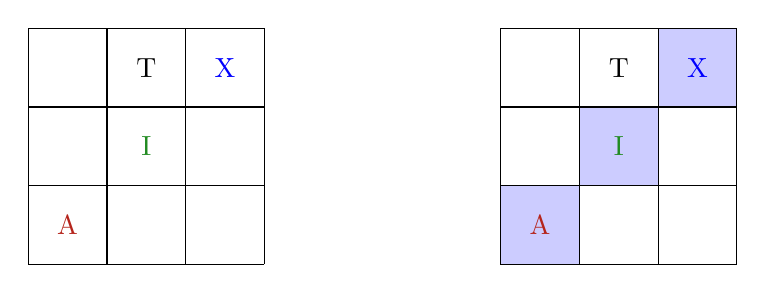
\begin{tikzpicture}
\draw[step=1cm,color=black,thin] (0,0) grid (3,3);
\node[BrickRed] at (0.5,0.5) {A};
\node[black] at (1.5,2.5) {T};
\node[ForestGreen] at (1.5,1.5) {I};
\node[blue] at (2.5,2.5) {X};

\draw[step=1cm,color=black,thin] (6,0) grid (9,3);
\filldraw[fill=blue!20!white, draw=black] (6,0) rectangle (7,1);
\filldraw[fill=blue!20!white, draw=black] (7,1) rectangle (8,2);
\filldraw[fill=blue!20!white, draw=black] (8,2) rectangle (9,3);
\node[BrickRed] at (6.5,0.5) {A};
\node[black] at (7.5,2.5) {T};
\node[ForestGreen] at (7.5,1.5) {I};
\node[blue] at (8.5,2.5) {X};
\end{tikzpicture}
\caption{Example of a challenge-response. The left matrix is the challenge and the right the response, where the blue squares are the ones selected by the user.}
\label{fig:ex1}
\end{figure}

\paragraph{Risk analysis} We chose to draw an attack tree as a risk analysis of our authentication method. The attack goal is to access the chat without a valid account. The entire tree is represented in Figure~\ref{fig:attacktree}.
We used the labels \textcolor{ForestGreen}{Possible} and \textcolor{BrickRed}{Impossible}, making the assumption that the chat RP, the OpenID OP and the users are on separate machines and servers. We did not use cost or probability estimates, because these would highly depend on the actual usage of the system.
\todo[inline]{explain tree}
The tree contains the major threats we were able to identify for the system. Two particular items need some explanation.
\begin{itemize}
\item All the possibilities in the subtree \texttt{Log in to chat $\rightarrow$ Get login $+$ password $\rightarrow$ From machine} are labeled as impossible. Spying on the screen or using a key logger once do not reveal the secret, as each challenge requires a customised response. They become possible however if used repeatedly until a statistical analysis of the data makes it possible to deduce the secret. The impossible label in this case stands for an effort we have estimated as too time consuming as it would only reveal a single login. The database is different as it contains all accounts. We have added the leaf ``Decrypt DB'' although it is not encrypted as it is now; because the risk analysis comes to the conclusion that accessing it is already impossible, encrypting it is not needed to make an attack impossible, which is why it can stay unencrypted.
\item The dictionary attack in the subtree \texttt{Log in to chat $\rightarrow$ Crack the system $\rightarrow$ Guess password} is labeled as impossible for the same reason as mentioned above: it would require a lot of time due to the repetitions that are necessary to gather useful statistical data. Every password has to be used enough times to make sure that it does not apply to a given user. This effect is however somewhat limited by the fixed length of the password.
\end{itemize}
\begin{figure}
\centering
\includegraphics[width=1.1\textwidth]{attacktree.pdf}
\caption{Attack tree of our own authentication method.}
\label{fig:attacktree}
\end{figure}
As we can see in the tree, the final conclusion is that an intrusion is possible both by acquiring a login and password and by cracking the system. As in most authentication systems, the user itself is a major security threat. We identified bribing and asking (with some social engineering) as the main threats which involve human users. The second major threat is the backdoor.
We concluded that SQL injection and eavesdropping on the network are both possible. Several methods can mitigate SQL injections: prepared statements and restricted permissions have proven efficient. Despite these measures, we still think of the attack as possible because it primarily concerns our way of handling the database, which may be error-prone.
The replay attack seemed possible to us due to the lack of tokens in the communication between the user and the OpenID OP.

% compare to passwords

\paragraph{Use-case diagram} The use case diagram, represented in Figure~\ref{fig:usecasedia} of our authentication mechanism depicts the interactions between the user and the system. It does not take the OpenID mechanism into account and only deals with plain authentication, thus not representing further functionalities.
\begin{figure}
\centering
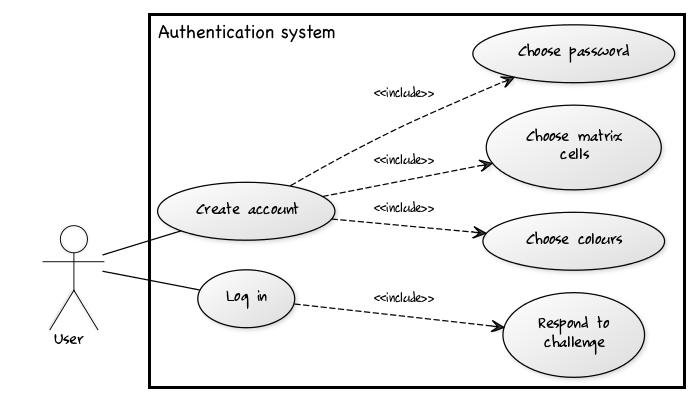
\includegraphics[width=0.8\textwidth]{usecasedia.png}
\caption{Use case diagram of our authentication method [created with \url{www.yuml.me}].}
\label{fig:usecasedia}
\end{figure}


\paragraph{Sequence diagram} The sequence diagram of our authentication mechanism is represented in Figure~\ref{fig:seqdia}. We do not consider the OpenID mechanism in it.
\begin{figure}
\centering
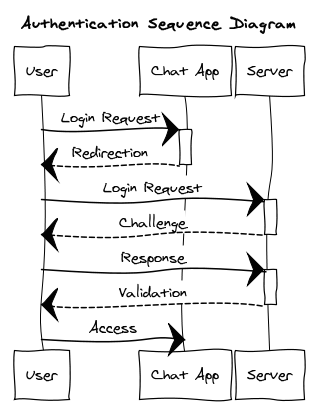
\includegraphics[width=0.6\textwidth]{seqdia.png}
\caption{Sequence diagram of our authentication method [created with \url{www.websequencediagrams.com}.}
\label{fig:seqdia}
\end{figure}

\clearpage

\subsection*{Implementation of an authentication method}
\paragraph{Overview}
% how to implement

\paragraph{Database}
The user table \texttt{OPUserTable} needs to be changed in the database.
An attribute that contains the selected matrix positions and another one for the selected colours need to be added to remember the users credentials.
An additional attribute has to be there: the expected response value. Once the server issues a challenge, it has to remember what response a given user should send back next. This is stored and deleted as soon as a response from the user is received, whether correct or not, as in both cases the next challenge will be a new one.

\paragraph{User interface}
The authentication is performed in four steps:
\begin{itemize}
\item The user can enter a username;
\item the server generates a challenge and presents it to the user;
\item the user enters his response;
\item the server checks the response and either redirects the user or denies access.
\end{itemize}
The user interface needs to have one more page. The first authentication page will only have a username field.  When the username is submitted, another page with the challenge and an answer field will appear. Once the answer to the challenge is entered correctly, the current user page will appear and the application will continue as it is now.

\paragraph{HTML and CSS}
First of all, we have to remove the password field from the original login page.

After that, another HTML page is needed. A copy of the \texttt{logIn.html} with small modifications will suffice. Instructions for the challenge need to be added with, of course, the challenge image will replace the current username
field.

Finally, a little CSS will be added for the instructions text and the challenge image.

\todo[inline]{clarify?? modified login + new page with challenge AND modified sign up}

\paragraph{Servlets}
A new servlet will be added to generate the challenge image. It will generate the challenge and then use the id of the user in the url as input for
calculating the answer based on the user's secret and store it as the next expected answer in the user table of the database.

\paragraph{OpenIDA}

\paragraph{Security flaws}
% clear passwords: fix = encrypt everywhere (e.g. hash)
% replay attack between the user and OpenIDA: fix = use tokens in this step

\end{document}
